\chapter{基督對祂的教會說話（2:1-3:13）}
\normalsize
\section{先了解初代教會的時代背景}

寫啟示錄的約翰所處的年代，正是羅馬帝國最強盛的時期之一。地上的君王，似乎無可匹敵。
也就在這個年代，初代教會誕生。他們認識真正的君王基督，並且為真理作見證，甚至至死不渝。

羅馬帝國高度集權，皇帝的權威遍及帝國各地。皇帝崇拜也逐漸成為帝國公共生活的一部分。不過，各地的宗教政策並不完全一致；只要不被視為威脅帝國秩序，許多民族仍可以保留自己的傳統宗教。猶太教歷史悠久，在羅馬統治下可以享有一定程度的宗教特權，因此猶太人通常可以按照祖先的律例敬拜上帝。基督教起初從猶太教的背景中發展出來，在一些地方也被視為猶太傳統中的一個群體；但隨著基督教逐漸與猶太教分離，這種既有的宗教身分的保護傘也就減弱了。\footnote{Beale, G. K. (1999).}

基督徒敬拜獨一真神，宣認耶穌基督是真正的主，因而不能把皇帝當作神來敬拜。這使他們遭受社會敵意與官方壓力，甚至在某些地區面臨財產被沒收、流放或處死的危險。

我畫出了西元1年至138年的皇帝時間軸。圖\ref{fig:roman_emperors}可以讓我們可以看見這段時期羅馬政權的更迭。
其中，尼祿（Nero）與圖密善（Domitian）在歷史上常被稱為暴君。兩人都集中皇權、壓制政敵、處決反對者，也曾以叛國罪等罪名打擊政敵。尼祿尤其因西元64年羅馬大火後迫害基督徒而聞名。
見表\ref{tab:nero-domitian-zh}。
\footnote{至於圖密善，古代資料記載他鎮壓異議者，但是否曾大規模地迫害基督徒，仍有不同看法。}



\begin{figure}[htbp]
    \centering
    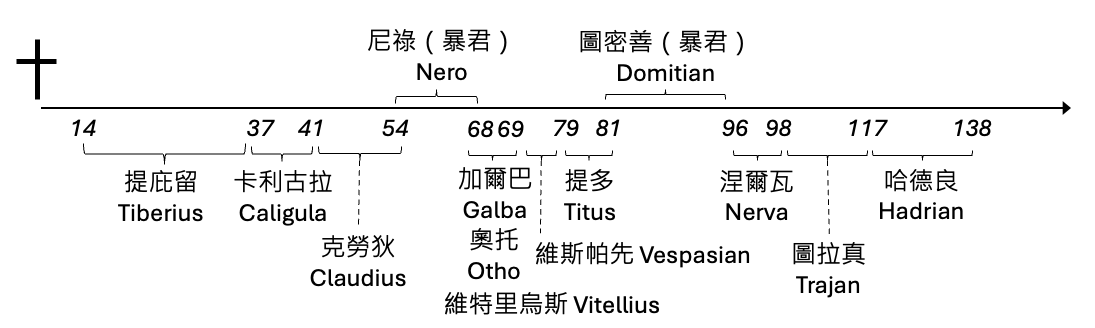
\includegraphics[width=\textwidth, trim=0 0 0 0, clip]{images/roman_emperors.png}
    \caption{西元1年至138年的羅馬皇帝時間軸}
    \label{fig:roman_emperors}
\end{figure}





\clearpage
{
\small
\begin{longtable}{|p{2.5cm} | p{6.5cm}|}
\caption{尼祿、圖密善} 
\label{tab:nero-domitian-zh} \\
\hline 
\textbf{人物} \footnote{此尼祿肖像現位於慕尼黑雕塑館，圖密善肖像現位於法國羅浮宮。} &
\textbf{迫害} \\
\hline
\centering
尼祿（Nero）\\
\includegraphics[
    width=\linewidth,
    trim=0 0 0 0, 
    keepaspectratio
]{images/nero.jpg}

&
\vspace{-0.3cm}
\begin{itemize}[nosep, leftmargin=10pt]
\item 處決政敵與元老院議員。
\item 以叛國罪等法律打擊政敵。
\item 下令殺害自己的母親阿格里皮娜（Agrippina）。
\item 羅馬大火（64 年）後迫害基督徒。
\item 以恐懼、暴力和專斷的手段統治。
\item 拒絕參與帝國崇拜者可以被控為「不敬神」（atheism）。
\end{itemize}
\\[-0.5cm]
\hline

\centering
圖密善\\
（Domitian）\\
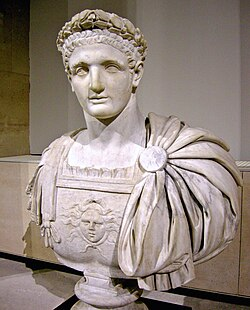
\includegraphics[
    width=\linewidth,
    keepaspectratio
]{images/domitian.jpeg}

&
\vspace{-0.3cm}
\begin{itemize}[nosep, leftmargin=10pt]
\item 處決元老院議員及政敵。
\item 以叛國罪等法律打擊政敵。
\item 沒收被定罪政敵的財產。
\item 要求以「主與神」（Dominus et Deus）稱呼他。此稱呼在書面和口頭上都不可更改。\footnote{Suetonius. (1914). Lives of the Caesars: Volume II (J. K. Rolfe, Trans.). Harvard University Press.}
\item 拒絕參與帝國崇拜者可以被控為「不敬神」（atheism）。
\item 透過猜疑、告密與壓制來統治。
\end{itemize} 
\\
\hline
\end{longtable}
} 

了解此逼迫嚴峻的時代，我們來讀耶穌給七個教會的書信。七個教會的位置，可以參照圖\ref{fig:turkey-seven-churches}。
\normalsize
\subsection{為什麼是此七間教會？}

讀者的第一個問題，可能是為什麼是此七間教會？新約書信還提到羅馬、哥林多、腓立比、歌羅西、帖撒羅尼迦等許多教會，怎麼沒有在其中？
這七間教會之所以出現在啟示錄中，並不是約翰自行挑選的，而是基督吩咐約翰的：「你所看見的，當寫在書上，達與亞細亞的七個教會」。
「七」是啟示錄中反覆出現、表達完整性的數字。因此，這七封書信不只是給這七間教會，每封書信最後都以「聖靈向眾教會所說的話，凡有耳的，就應當聽」作結。這表示基督對一間教會所說的話，也是在向眾教會說話。

為了讓讀者更貼近當時的處境，我特別設計了「弟兄對話」，讓我們彷彿走進這七間教會，在聽見基督說話以前，先聽見弟兄姊妹如何看待自己的教會，以及他們所處的環境。

這七封書信都有基督對各教會的稱許、責備、命令和應許。我也將基督的信息分為「基督的稱許」、「基督的責備」、「基督的命令」和「基督的應許」四個部分。
特別值得注意的是，其中有兩間教會的「基督的稱許」標示為「沒有」。「沒有」這兩個字何等令人警醒，也何等令人心痛。若主親自對我們的教會說話，我們是否也能聽見祂的稱許？還是我們也只能面對一個令人心痛的「沒有」？

\section{以弗所教會(2:1-7)}

\begin{DialogueBox}
\noindent\faUser\ 弟兄一：「我們以弗所的弟兄們，向來看重主的道。有人傳講異樣的教訓，我們便察驗；有人自稱使徒，我們也不輕易接納。這些年來，眾弟兄為主的名勞苦，忍耐逼迫，也沒有因患難退後。我想，我們既如此持守主的道，又忠心服事，求主悅納我們的工作。」

\noindent\faUser\ 弟兄二：「我們確實為主的名作了許多工。只是……我有時想起我們初信主的日子，那時弟兄姊妹熱切相愛，聽道、禱告、擘餅。如今我們仍然持守真道，也仍然殷勤作工，只是不知不覺間，我們裡面起初愛主、愛弟兄的心，是否已不如從前了？」
\end{DialogueBox}

\subsection{地理背景}
以弗所教會所在的以弗所城，是一座繁華而深受偶像崇拜影響的城市。
今天如果前往以弗所古城參觀，仍然可以看到以弗所大劇場、海港大道、大理石大道、古代市集廣場、圖書館、神殿與噴泉等遺址。走在這些保存至今的遺跡之間，我們仍能想像當年以弗所作為羅馬帝國重要城市之一的繁華景象。

以弗所的大亞底米神廟（Temple of Artemis）是以弗所城市身分的重要象徵。大亞底米（Artemis）是希臘名稱，羅馬人稱她為 Diana（戴安娜）。對亞底米的崇拜不只是宗教活動，也帶動了相關的商業與手工業。使徒行傳19:24記載，銀匠底米丟「為亞底米製造銀龕」，使許多工匠因此獲利。

然後保羅一行人在以弗所傳講福音，許多人離棄偶像歸向基督。福音的傳播改變了人的生命，因此也開始影響以偶像崇拜為中心的社會與經濟活動。於是，銀匠底米丟聚集其他銀匠和相關工匠，指控保羅一行人威脅亞底米的尊榮，使他們的生意受到影響。結果，整座城都轟動起來。眾人湧進大劇場，約有兩個小時不住地喊著：「大哉！以弗所人的亞底米啊！」
路加醫生也不減幽默，他記著：「聚集的人、紛紛亂亂、有喊叫這個的、有喊叫那個的、大半不知道是為甚麼聚集。」（使徒行傳19:28,32,34）

想像一下，當時眾人聚集在巨大的劇場中，持續兩個小時高聲呼喊。這不僅讓我們看見以弗所城市的規模，也讓我們感受到他們的宗教熱情，以及偶像崇拜在城市生活中的重要地位。

正是在這樣一座繁華、富庶，又深受偶像崇拜影響的城市中，基督建立了祂的教會。
以弗所教會是蒙受豐富恩典的教會。保羅給以弗所教會的書信，一開始就是偉大的揀選論：「神從創立世界以前、在基督裡揀選了我們。」（以弗所書1:4)並且說明神在基督裡所成就的偉大奧秘。
這奧秘就是教會。就是「外邦人在基督耶穌裡、藉著福音、得以同為後嗣、同為一體、同蒙應許。」（以弗所書3:6）。他更為他們禱告，使基督因他們的信住在他們心裡，使他們的愛心「有根有基」，並且「能以和眾聖徒一同明白基督的愛，是何等長闊高深」（以弗所書3:17–18）。以弗所教會知道神永恆的揀選，明白福音的奧秘，在基督裡得著豐富的恩典，也有信心和愛心。


\subsection{基督的稱許}

\begin{ScriptureBox}

\item[2:1] 你要寫信給以弗所教會的使者、說、那右手拿著七星、在七個金燈臺中間行走的、說、

\item[2:2] 我知道你的行為、勞碌、忍耐、也知道你不能容忍惡人、你也曾試驗那自稱為使徒卻不是使徒的、看出他們是假的來。

\item[2:3] 你也能忍耐、曾為我的名勞苦、並不乏倦。

\end{ScriptureBox}

這是一群身體力行的信徒。他們為主勞碌、忍耐，持守真道，分辨是非。保羅與他們告別時，以弗所教會眾長老流淚痛哭，最令眾長老傷心的，是保羅所說：「以後不能再見我的面」（使徒行傳20:38）。
保羅更鄭重的勸他們警醒，因為「必有兇暴的豺狼進入你們中間，不愛惜羊群」（使徒行傳20:29）。這是一群有真理、有勞苦、有忍耐，也有愛的信徒。

\subsection{基督的責備}

\begin{ScriptureBox}

\item[2:4] 然而有一件事我要責備你、就是你把起初的愛心離棄了。

\end{ScriptureBox}

然而，約三十多年後，基督透過約翰向這間教會說「你把起初的愛心離棄了。」

從第一代的基督徒，到此時，教會中可能已經有了第二、第三代的信徒。真理的教導，教會的事奉，和會眾忍耐的品格都在。從人的眼光來看，這真是眾教會的榜樣。
可是有一份元素漸漸在流逝了，那就是起初的愛。這正是以弗所教會最值得我們思想的地方：一間可以為真理站立、為主勞苦、忍耐到底的教會，仍然可能在不知不覺中失去起初的愛。

\subsection{基督的命令}

\begin{ScriptureBox}

\item[2:5] 所以應當回想你是從那裡墜落的、並要悔改、行起初所行的事．你若不悔改、我就臨到你那裡、把你的燈臺從原處挪去。

\item[2:6] 然而你還有一件可取的事、就是你恨惡尼哥拉一黨人的行為、這也是我所恨惡的。

\end{ScriptureBox}

冷淡了的愛心，如何回到最初？答案是：悔改。
悔改使冷淡的心重新被主喚醒，使失落的愛重新燃起。即使我們已經走了很遠的路，恩典仍然可以使我們回轉，使我們在主裡日新又新。
悔改不是單單為過去的失敗感到難過，而是重新轉向基督，回到起初愛祂、跟隨祂的生命。
我們需要天天悔改，就是主耶穌吩咐的，「天天背起自己的十字架來跟從我。」（路加福音 9:23）


值得注意的是，基督對以弗所教會的責備，並不表示他們在真理上已經妥協。相反地，他們仍然恨惡尼哥拉一黨人的行為，這一點也是基督所肯定的。關於「尼哥拉一黨」究竟是什麼人，我們今天並不能確定其具體背景與教導。 \footnote{MacArthur, J. (2007).} 然而，他們所代表的，是一種基督所恨惡的錯誤教導與行為。

\subsection{基督的應許}

\begin{ScriptureBox}

\item[2:7] 聖靈向眾教會所說的話、凡有耳的、就應當聽。得勝的、我必將　神樂園中生命樹的果子賜給他喫。

\end{ScriptureBox}

這裡的「生命樹」明顯把我們帶回創世記2–3章。而「樂園」對應啟示錄22:1–5。因此，從創世記到啟示錄，我們可以看見：人是從伊甸園的失落，到基督裡的救贖，到得勝者進入神的樂園，到新天新地中的完全同在。基督不只是呼召祂的教會在地上忠心到底；祂最終要把屬祂的人帶入榮耀裡。
今天教會所面對的爭戰、悔改、忍耐與忠心，都不是救贖故事的終點；終點乃是進入神永恆的同在。所以，基督給以弗所教會的應許，既回應了他們當下的光景，也把他們的眼目帶向最後的榮耀。

\section{士每拿教會(2:8-2:11)}

\begin{DialogueBox}
\noindent\faUser\ 弟兄一：「我們士每拿，按著世人的眼光看，是困苦貧窮的。有人因信主的緣故受人毀謗，有人因不肯隨從眾人去稱君王是神，而失去生計。已有弟兄為主的名捨了性命。然而，雖是如此，我們仍聚集在一起敬拜主。若能持守基督的名，地上的貧窮又算得甚麼呢？」

\noindent\faUser\ 弟兄二：「我們在世人眼中或許一無所有，但有一樣，是無論如何也不可失去的，就是對主的忠心。將來所要面對的苦楚，也許比今日更深；但我們既已歸屬基督，就當持守到底。」
\end{DialogueBox}

\subsection{地理背景}

士每拿，是今天土耳其第三大城市伊茲米爾（İzmir），也是愛琴海沿岸的重要港口城市。今日仍可看見許多不同時代留下的歷史痕跡，包括古代市集廣場（Agora），羅馬時期的柱廊、公共建築與城市基礎設施。

士每拿在羅馬時代，就是忠誠於羅馬的重要城市。早在主前約195年，士每拿便建立了獻給「羅馬」（Roma）的神廟，表達對羅馬的忠誠。到了主後26年，士每拿又在與其他亞洲城市的競爭中獲准建立獻給提比留皇帝、莉薇亞以及羅馬元老院的神廟。

在這樣的背景下，基督徒拒絕參與皇帝崇拜，就可能被視為拒絕履行忠誠。對士每拿的基督徒而言，心裡相信並口裡承認「耶穌是主」，是一個關乎生命的事情。所以我們更能了解主耶穌對士每拿教會的稱許是何等寶貴。



\subsection{基督的稱許}

\begin{ScriptureBox}

\item[2:8] 你要寫信給士每拿教會的使者說、那首先的、末後的、死過又活的說、

\item[2:9] 我知道你的患難、你的貧窮、（你卻是富足的）也知道那自稱是猶太人所說的毀謗話、其實他們不是猶太人、乃是撒但一會的人。

\end{ScriptureBox}

士每拿教會一直保持此至死忠心的優良美德。約在主後155–160年間，坡旅甲（Polycarp）是士每拿教會的監督，坡旅甲年輕時曾到以弗所，接受使徒約翰的教導。他被捕並被帶到官府面前。根據《坡旅甲殉道記》\footnote{\textit{Martyrdom of Polycarp}. (1885). (A. Roberts \& J. Donaldson, Trans.).
Christian Literature Publishing. (Original work published ca. 155)}，當他被要求否認基督時，他回答：「我服事祂八十六年，祂從未虧負我；我怎能褻瀆那拯救我的王？」他也是早期基督教最著名的殉道見證之一。士每拿是一座以忠於羅馬而聞名的城市；基督卻在這座城市中建立了一群只以基督為王的子民。

\subsection{基督的責備}

沒有。

\subsection{基督的命令}

\begin{ScriptureBox}

\item[2:10a] 你將要受的苦你不用怕．魔鬼要把你們中間幾個人下在監裡、叫你們被試煉．你們必受患難十日。你務要至死忠心、

\end{ScriptureBox}

這裡的十日，表明是一段短的日子。患難有期，非無限期並失控的苦難。

\subsection{基督的應許}

\begin{ScriptureBox}

\item[2:10b] 我就賜給你那生命的冠冕。

\item[2:11] 聖靈向眾教會所說的話、凡有耳的、就應當聽。得勝的、必不受第二次死的害。

\end{ScriptureBox}

「第二次的死」指的是末後的審判與永遠的刑罰（啟示錄20:14）。這裡的「得勝」，不是說信徒靠自己的忠心賺取救恩，而是指屬基督的人在患難中持守信仰，靠著基督的恩典忠心到底。
對士每拿教會而言，這個應許尤其寶貴。他們因忠於基督而殉道。但肉身的死亡並不能改變基督所賜的永恆生命。那位「死過又活的」基督已經勝過死亡，因此屬祂的人不受第二次死的害。他們可能失去今生的生命，卻不會失去基督所賜的永恆生命。

\section{別迦摩教會(2:12-2:17)}

\begin{DialogueBox}
\noindent\faUser\ 弟兄一：「別迦摩是何等繁盛的城，眾多神廟林立，祭祀之事日日不息。只是，城中的人設席祭祀，邀請我們同席，我們無法拒絕。是否只要守住所信的，其他稍作退讓，也可以吧？」

\noindent\faUser\ 弟兄二：「我也曾如此想過。有些弟兄說，只要心裡仍信靠基督，偶爾赴席、吃祭偶像之物，也可以。可是近來我心裡越發不安……我們原是蒙召離開偶像歸向主的。若一次又一次向這些事退讓，我們究竟是在保守自己，還是在一步一步偏離主的道呢？」
\end{DialogueBox}


\subsection{地理背景}

別迦摩（Pergamum）就是今天土耳其西部的貝爾加馬（Bergama），位於伊茲密爾省（Izmir Province），今日的古城遺址已列入世界文化遺產。今日來到貝爾加馬，可以看到別迦摩的衛城（Acropolis），位於山丘頂端，可以看到古代劇場、雅典娜神廟、圖書館、宙斯祭壇遺址，以及羅馬帝國君王圖拉真神廟。阿斯克勒庇翁（Asclepion）：古代著名的醫療與治療中心，也是別迦摩最重要的羅馬時期遺址之一。別迦摩以圖書館與羊皮紙（parchment）聞名，是古代重要的知識中心。它羅馬時期則成為亞細亞行省的重要城市，並具有帝國崇拜中心的功能。

\begin{figure}[htbp]
    \centering
    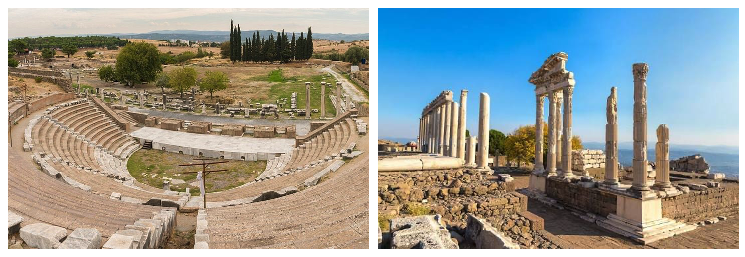
\includegraphics[
    width=1\textwidth, 
    trim=0 0 0 0, 
    clip]{images/pergamum3.png}
    \caption{別迦摩古代劇場、宙斯祭壇遺址}
    \label{fig:pergamum3}
\end{figure}

\subsection{基督的稱許}

\begin{ScriptureBox}

\item[2:12] 你要寫信給別迦摩教會的使者、說、那有兩刃利劍的說、

\item[2:13] 我知道你的居所、就是有撒但座位之處．當我忠心的見證人安提帕在你們中間、撒但所住的地方被殺之時、你還堅守我的名、沒有棄絕我的道。

\end{ScriptureBox}

別迦摩不只是文化與知識的中心，也是一座具有濃烈宗教與帝國崇拜氣氛的城市。 因此，2:13稱為「有撒但座位之處」。

\subsection{基督的責備}

\begin{ScriptureBox}

\item[2:14] 然而有幾件事我要責備你、因為在你那裡、有人服從了巴蘭的教訓．這巴蘭曾教導巴勒將絆腳石放在以色列人面前、叫他們喫祭偶像之物、行姦淫的事。

\item[2:15] 你那裡也有人照樣服從了尼哥拉一黨人的教訓。

\end{ScriptureBox}

在民數記25章，巴蘭引誘以色列人與摩押女子發生不正當的性淫亂，和陷入偶像崇拜，使他們得罪神。

以色列人在異教環境中，因為妥協而陷入偶像崇拜與淫亂。所以這裡是在告訴別迦摩教會，你們現在所面對的問題，並不是一個全新的問題。
這個問題以色列在曠野曾經面對過，而你們正在重演那個故事。
應用在今日，這如同是「妥協性的教導和門徒訓練」。是我們應當謹慎的。

\subsection{基督的命令}

\begin{ScriptureBox}

\item[2:16] 所以你當悔改、若不悔改、我就快臨到你那裡、用我口中的劍、攻擊他們。

\end{ScriptureBox}
如第一章表\ref{tab:christ-revelation-1-3}，基督口中利劍代表祂以真理審判錯謬。所以這裡是呼召教會離開錯誤的教導和行為，重新忠於基督。

\subsection{基督的應許}

\begin{ScriptureBox}

\item[2:17] 聖靈向眾教會所說的話、凡有耳的、就應當聽。得勝的、我必將那隱藏的嗎哪賜給他．並賜他一塊白石、石上寫著新名．除了那領受的以外、沒有人能認識。

\end{ScriptureBox}

嗎哪首先讓人想到以色列人在曠野中所吃的嗎哪（出埃及記16:15）。別迦摩教會在這個充斥異教崇拜的敵對環境，基督卻應許得勝者有另一種「食物」。不是向偶像妥協所得到的東西，而是從基督而來的真正生命供應。

這裡「白石」最好的理解似乎是按照羅馬人的習俗來解釋這塊「白石」。在競技比賽中，勝利者會獲頒白石。白石上刻有運動員的名字，並作為他參加特別頒獎宴席的入場券。\footnote{MacArthur, J. (2007). }
「新名」在聖經裡常常涉及新的身分、與神新的關係，所以，這裡的應許是，忠於基督的人，基督要以更深的生命供應和新的身分來代替。

\section{推雅推喇教會(2:18-29)}

\begin{DialogueBox}
\noindent\faUser\ 弟兄一：「我們推雅推喇的弟兄姊妹，殷勤服事，彼此相愛，又有信心和忍耐。近來開辦的慈善事工，也比從前更加增長。我們又透過參與城中各行各業的聚會，積極傳福音、幫助鄰舍。我想，只要我們一面持守對主的忠心，一面與眾人和睦相處，豈不是也能在這城中為主作美好的見證嗎？」

\noindent\faUser\ 弟兄二：「我也盼望如此。只是，有些事情實在叫我心裡不安。各行各業聚會的時候，常常會有向偶像獻祭的事情。我們教會甚至邀請那個自稱為先知的婦人耶洗別來教導。她勸說，信徒也可以吃祭偶像之物。」
\end{DialogueBox}


\subsection{地理背景}

推雅推喇（Thyatira／Thyateira）位於今天的土耳其西部的阿克希薩爾（Akhisar）。它不是以宏偉的政治地位或大型宗教中心聞名，而是以商業和手工業著稱。考古發現顯示，推雅推喇有非常多不同的行會（guilds），包括羊毛工人，染布工人，亞麻工人，皮革工人，銅匠等等。使徒行傳16:14 中的呂底亞（Lydia）就是一個賣紫色布匹的推雅推喇城的人。她在腓立比遇到保羅，後來成為基督徒。這些行會不只是單純的職業協會，同時也具有社交、向城市的神明獻祭或宗教宴席。此地行會工藝精湛，「腳像光明的銅」正可能是引用當地的銅匠的銅藝。這裡的銅，是一種由銅與鋅混合而成的合金，是一種較為純淨、精煉的黃銅。推測這類金屬是由推雅推喇（Thyatira）當地的工匠行會為軍事用途所製造。\footnote{Osborne, G. R. (2002).}

\subsection{基督的稱許}

\begin{ScriptureBox}

\item[2:18] … 那眼目如火焰、腳像光明銅的　神之子、說、

\item[2:19] 我知道你的行為、愛心、信心、勤勞、忍耐．又知道你末後所行的善事、比起初所行的更多。

\end{ScriptureBox}

\subsection{基督的責備}

\begin{ScriptureBox}

\item[2:20] 然而有一件事我要責備你、就是你容讓那自稱是先知的婦人耶洗別教導我的僕人、引誘他們行姦淫、喫祭偶像之物。

\item[2:21] 我曾給他悔改的機會、他卻不肯悔改他的淫行。

\item[2:22] 看哪、我要叫他病臥在床、那些與他行淫的人、若不悔改所行的、我也要叫他們同受大患難。

\item[2:23] 我又要殺死他的黨類、〔黨類原文作兒女〕叫眾教會知道、我是那察看人肺腑心腸的．並要照你們的行為報應你們各人。

\end{ScriptureBox}

耶洗別是北國以色列王亞哈的外邦王后，積極推動巴力崇拜、逼迫耶和華的先知，並因悖逆上帝而成為聖經中邪惡與淫亂的象徵。（列王紀上17–21章）。約翰刻意把一個當代教會中的人物稱為「耶洗別」，使讀者透過舊約人物來理解當前教會的問題。
這裡的「行姦淫、喫祭偶像之物」包括實際的異教祭祀以及社會生活中的宴席。在舊約中，「淫亂」又經常成為以色列背離耶和華、追隨偶像的象徵語言。
因此，這段經文的核心問題是教會是否仍然忠於基督，還是為了與周圍的文化、宗教、權力結合而妥協？

\subsection{基督的命令}

\begin{ScriptureBox}

\item[2:24] 至於你們推雅推喇其餘的人、就是一切不從那教訓、不曉得他們素常所說撒但深奧之理的人．我告訴你們、我不將別的擔子放在你們身上。

\item[2:25] 但你們已經有的、總要持守、直等到我來。

\end{ScriptureBox}
這裡的「撒但深奧之理」有兩種可能的解釋：\footnote{Osborne, G. R. (2002); Beale, G. K. (1999).}
\begin{enumerate}
\item 諷刺性的說法：這可能是在諷刺耶洗別所聲稱自己「知道神深奧之事」（參歌林多前書 2:10）。
\item 按字面理解：耶洗別可能是根據某種諾斯底主義（gnostic）\footnote{諾斯底思想主張物質世界是邪惡的、唯有靈魂才是良善的，並認為人得救是靠獲得隱祕的屬靈「知識」（希臘文 gnōsis），而非單靠信心與恩典。使徒約翰在他的書信中，指出受了諾斯底思想的假教師與假福音的謬誤。
詳見「被恩典追上」第七章「關於諾斯底主義（Gnosticism）」。}
的原則教導：基督徒應當經歷「撒但深奧之理」，藉此勝過撒但。這些活動，親身經歷異教的「深處」。
\end{enumerate}
第一種解釋似乎更為可能，尤其是它對應2:9。在那裡，猶太人的反對者被稱為「撒但一會」。有趣的是，這兩種解釋都與諾斯底主義的教導有關。諾斯底主義簡單說，就是認為人藉著獲得特殊、隱秘的「知識」（gnosis），就能認識真正的神、脫離物質世界，並得著救贖的一種思想。按照第一種理解，「神深奧之事」指的可能是原始諾斯底主義所追求的深奧、祕傳的知識（gnosis）。按照第二種理解，則可能涉及一群諾斯底式放縱主義者（約翰一書1:8–10；3:9）。這些人認為，由於自己擁有特殊的「知識」，即使參與罪惡的活動，也不會真正成為罪。

\subsection{基督的應許}

\begin{ScriptureBox}

\item[2:26] 那得勝又遵守我命令到底的、我要賜給他權柄制伏列國．

\item[2:27] 他必用鐵杖轄管他們、〔轄管原文作牧〕將他們如同窰戶的瓦器打得粉碎．像我從我父領受的權柄一樣．

\item[2:28] 我又要把晨星賜給他。

\item[2:29] 聖靈向眾教會所說的話、凡有耳的、就應當聽。

\end{ScriptureBox}

承接上文，「得勝」是在面對「耶洗別」的教訓、偶像崇拜和妥協時，仍然持守基督的命令到底。

「鐵杖」是使用了詩篇2:8–9：「你求我，我就將列國賜你為基業……你必用鐵杖打破他們。」這裡不是說信徒自己成為另一位基督，而是說
基督從父領受的權柄然後與得勝者分享。得勝者與基督一同掌王權。希臘原文「轄管」是牧養、照管、治理的意思。因此這個王權不是暴力性的脅迫統治毀滅，而是君王治理。

「晨星」在啟示錄後面會得到非常重要的解釋，是基督自己。「我是……明亮的晨星。」（22:16）因此「把晨星賜給他」最終是指向基督自己。所以最大的賞賜不只是「權柄」，而是基督自己成為得勝者的賞賜。

推雅推喇教會讓我們學習到，教會之所以必須拒絕「耶洗別」，是因為羔羊已經用自己的血買贖了屬祂的人，並且要將屬祂的人帶入榮耀中。既然羔羊配得敬拜，教會就不能把忠誠分給偶像，而應當持守對基督的忠誠，直到祂帶領祂的教會進入榮耀裡。

\section{撒狄教會(3:1-6)}


\begin{DialogueBox}
\noindent\faUser\ 弟兄一：「我們撒狄教會如今頗有名聲。每逢聚會，弟兄姊妹聚集甚多；在城中，人也知道我們是屬基督的群體。看見眾人如此熱心，我心裡便想，我們必是為主作了不少工，主也必與我們同在。」

\noindent\faUser\ 弟兄二：「從外面看，確實如此。只是我心裡卻常有一個疑問：我們裡面的生命是否也同樣興盛呢？我們在主面前的禱告、彼此的勸勉，以及在罪中的悔改，是否已漸漸冷淡？人看我們是活的，在主眼中，我們又究竟是怎樣的光景呢？」
\end{DialogueBox}

\subsection{地理背景}

撒狄（Sardis）位於推雅推喇東南方約三十至四十英里。約於主前 1200 年建立，是古代最古老的城市之一，後來成為富裕而強大的呂底亞王國（Lydian kingdom）的首都。撒狄也透過商業與貿易累積了巨大的財富，並且是最早鑄造金幣和銀幣的城市之一。

撒狄曾經是一個強大的軍事城邦，很少在戰爭中失敗。撒狄早期最著名的君王之一，是主前七世紀的吉吉斯（Gyges）；他奠定了撒狄的財富與權勢。其子克羅伊斯（Croesus）更是權勢顯赫，甚至自信有能力進攻波斯的古列王（Cyrus）。

然而，接下來的幾個世紀，撒狄卻數度防守鬆懈，遭遇重要的因軍事失敗，並逐漸失去昔日的軍事與政治地位。雖然撒狄仍然保持一定的財富與商業繁榮，但昔日作為呂底亞強權首都的榮耀已逐漸成為歷史。到了西元一世紀，撒狄基本上已經成為一座「活在過去」的城市：它仍然擁有昔日輝煌所留下的財富、文化與聲望，卻已不再是過去那個強盛的軍事與政治中心。此外，撒狄擁有一個相當大的猶太社群，其歷史可以追溯到主前五世紀或四世紀。這個猶太群體在撒狄的城市生活中具有一定的重要性，也反映出當地不同文化與宗教群體之間長期的交會。\footnote{Osborne, G. R. (2002).}

\subsection{基督的稱許}

沒有。


\subsection{基督的責備}

\begin{ScriptureBox}

\item[3:1] 你要寫信給撒狄教會的使者、說、那有　神的七靈、和七星的、說、我知道你的行為、按名你是活的、其實是死的。

\end{ScriptureBox}

「按名」表示撒狄教會在人看來是一個有名聲的教會；但基督揭露其內在實況是失去真正屬靈生命的，「死的」教會。這剛好與上文的城市歷史介紹巧合對比。撒狄曾經有輝煌的名聲，卻逐漸活在過去。當然使徒約翰並不是因為城市歷史，而說此教會是死的。

\subsection{基督的命令}

\begin{ScriptureBox}

\item[3:2] 你要儆醒、堅固那剩下將要衰微的．〔衰微原文作死〕因我見你的行為、在我　神面前、沒有一樣是完全的。

\item[3:3] 所以要回想你是怎樣領受、怎樣聽見的．又要遵守、並要悔改。若不儆醒、我必臨到你那裡如同賊一樣．我幾時臨到、你也決不能知道。

\end{ScriptureBox}

撒狄教會所需要的，是「儆醒、堅固、回想、遵守、悔改」。雖然他們表面上仍然存在，但屬靈生命已經衰微；然而，他們仍然有「剩下的」。因此，基督呼召他們抓住尚存的屬靈生命，使它重新堅固起來。這是一個從死亡邊緣回轉的呼召。

\subsection{基督的應許}

\begin{ScriptureBox}

\item[3:4] 然而在撒狄你還有幾名是未曾污穢自己衣服的．他們要穿白衣與我同行．因為他們是配得過的。

\item[3:5] 凡得勝的、必這樣穿白衣．我也必不從生命冊上塗抹他的名．且要在我父面前、和我父眾使者面前、認他的名。

\item[3:6] 聖靈向眾教會所說的話、凡有耳的、就應當聽。

\end{ScriptureBox}

\section{非拉鐵非教會(3:7-13)}


\begin{DialogueBox}
\noindent\faUser\ 弟兄一：「我們非拉鐵非是一個小教會，力量也微小，在眾教會中實在算不得甚麼。然而，主的道，我們仍當持守；主的名，我們也不敢否認。外面的患難雖然不少，我們所能作的也有限，但只要主賜我們一點力量，我們便當忠心站立，不離開祂的道。」

\noindent\faUser\ 弟兄二：「是的，我們原沒有甚麼可誇的。我們所求的，不是人的稱讚，只願在主面前忠心。若主為我們開了一扇門，我們就憑著祂所賜的力量盡力而行。」
\end{DialogueBox}


\subsection{地理背景}
非拉鐵非（Philadelphia，今日土耳其的 Alaşehir），位於撒狄東南約三十英里，處於一條主要貿易路線上，也被稱為「通往東方的門戶」。它是七座城市中建立年代最晚的一座。它大約在主前 189 年以後建立。創建者可能是帕加馬王國的歐邁尼斯二世（Eumenes II）的弟弟阿塔羅斯二世（Attalus Philadelphus）。他對哥哥具有深厚的愛與忠誠。所以將自己的名號賦予這座城市，使這城被稱為「弟兄相愛之城」。像撒狄一樣，非拉鐵非位於重要的地質斷層帶，常有地震。活躍的火山使土地肥沃，尤其適合葡萄種植。所以葡萄農業興盛。

頻繁的地震卻使當地生活非常困難。主後 17 年摧毀撒狄的那場大地震，也幾乎夷平了非拉鐵非。城市的城牆經常出現裂縫；居民住在不安全的建築物中，並且在作任何計畫時都必須考慮地震的因素。由於主後 17 年地震造成的巨大破壞，羅馬皇帝免除了非拉鐵非五年的進貢義務，使他們能夠恢復經濟並重建城市。

不過主後 92 年，在多米善（Domitian）統治期間，又發生了一件對非拉鐵非不利的事件。皇帝可能為了鼓勵種植糧食以供應羅馬軍隊，也可能是因為當時發生饑荒，下令砍掉一半的葡萄樹，並禁止種植新的葡萄樹。這項命令嚴重打擊了當地經濟，因為種植穀物的收益不如葡萄，而當地的火山土壤也並不特別適合穀物生長。由於葡萄樹需要多年才能重新生長，這項命令在整個亞細亞省引起極大憤怒，對當地而言是一場災難。\footnote{Osborne, G. R. (2002).}



\subsection{基督的稱許}

\begin{ScriptureBox}

\item[3:7] 你要寫信給非拉鐵非教會的使者、說、那聖潔、真實、拿著大衛的鑰匙、開了就沒有人能關、關了就沒有人能開的、說、

\item[3:8] 我知道你的行為、你略有一點力量、也曾遵守我的道、沒有棄絕我的名．看哪、我在你面前給你一個敞開的門、是無人能關的。

\item[3:9] 那撒但一會的、自稱是猶太人、其實不是猶太人、乃是說謊話的、我要使他們來在你腳前下拜、也使他們知道我是已經愛你了。

\end{ScriptureBox}


這裡「拿著大衛的鑰匙」直接對應以賽亞書22:22：「我必將大衛家的鑰匙放在他肩頭上；他開，無人能關；他關，無人能開。」而且這裡的重點是「那」位有權開門的人，所以是對他們說話的基督。

「略有一點力量」是指此教會因為遵守主的道而有主話語給的屬靈的力量，而不是地上的政治或是經濟力量。

「自稱是猶太人」：那些人可能掛名有社會地位，可是他們是「撒但一會」，「說謊話的」。
 
\subsection{基督的責備}

沒有。

\subsection{基督的命令}

\begin{ScriptureBox}

\item[3:10] 你既遵守我忍耐的道、我必在普天下人受試煉的時候、保守你免去你的試煉。

\item[3:11] 我必快來、你要持守你所有的、免得人奪去你的冠冕。

\end{ScriptureBox}

持守，是因為「我必快來」，所以免得人奪去你的冠冕。這是何等的盼望！

這裡的「保守你免去你的試煉」，是支持「大患難」與「災前被提」（pretribulation rapture）的關鍵。
\footnote{MacArthur, J. (2007). Osborne, G. R. (2002).}見「附錄：附錄：何時被提」。

\subsection{基督的應許}

\begin{ScriptureBox}

\item[3:12] 得勝的、我要叫他在我　神殿中作柱子、他也必不再從那裡出去．我又要將我　神的名、和我　神城的名、（這城就是從天上從我　神那裡降下來的新耶路撒冷）並我的新名、都寫在他上面。

\item[3:13] 聖靈向眾教會所說的話、凡有耳的、就應當聽。

\end{ScriptureBox}

你曾經住在地震帶嗎？像是台灣就是在地震帶，地震一來，即使是現代的鋼筋結構的高樓，仍使人害怕鋼柱斷裂，高樓墜下。
非拉鐵非教會地處地震帶，「力量」又小，神給他們的應許包括堅固的，在「神殿中做柱子」，他們必定感同身受。基督的應許給他們極大的盼望和安慰，使他們的視線到達啟示錄22章的新耶路撒冷。如表\ref{tab:Philadelphia}。

{
\renewcommand{\arraystretch}{1}
\begin{longtable}{p{4cm} | p{4cm}}
\caption{給非拉鐵非教會的應許} \label{tab:Philadelphia} \\
\hline 
非拉鐵非城市 & 
天上的城市 \\
\hline
地上的城市 &
天上的新耶路撒冷 \\
城市常有地震 &
神的城永恆穩固 \\
人可能離開城市 &
得勝者不再出去 \\
地上身份會改變 &
神的名寫在身上 \\
羅馬的城市榮譽 &
神的城的身份榮耀 \\
\hline
\end{longtable}
}


\section{老底嘉教會(3:14-22)}



\begin{DialogueBox}
\noindent\faUser\ 弟兄一：「我們老底嘉實在蒙福。城中買賣興盛，家道也多豐足；我們靠自己的勞苦置產積業，衣食無缺，生活安穩。就連我們聚集敬拜，也不缺甚麼。既沒有太多患難，也不至於放縱自己，只要安安穩穩地持守信仰，彼此和睦，不是很好嗎？」

\noindent\faUser\ 弟兄二：「我們的確甚麼都不缺。只是，我們不需要為生活掙扎，也不需要為信仰付出太多代價。我們是不是已經太習慣這樣安逸的日子了？」
\end{DialogueBox}

\subsection{地理背景}

老底嘉位於小亞細亞西部的弗呂家（Phrygia），它坐落在利庫斯（Lycus）河谷，地理位置優越，是連接東西方的重要交通與商業中心。

往東方約十英里有歌羅西（Colosse）。往北方約六英里有希拉波立（Hierapolis）。老底嘉因交通便利而非常富裕，主要發展商業與金融。其中最著名的是當地出產的黑羊毛，此羊毛柔軟、烏黑如烏鴉。因而老底嘉的紡織業超越了該地區其他服裝製造商。

老底嘉並以醫療產業著稱。有一所著名的醫學院，與米恩．卡魯（Men Karou，「河谷之神」）的神廟有關；此神祇被視為醫治之神。跟隨赫羅菲羅斯（Herophilos）醫學思想的人相信，可以使用複合藥物治療複雜疾病。他們還研發了一種治療眼疾的複合藥物，稱為「弗呂家粉末（Phrygian powder）」，使老底嘉獲得更大的聲望與財富。所以啟示錄3:18說：「買眼藥擦你的眼睛、使你能看見」，對老底嘉教會的人應該是很深刻的。當然，雖然我們不一定有老底嘉教會當地人的背景，可是我第一次讀到買眼藥能看見的比喻，也是一看就懂的。

老底嘉也在地震帶。主後 60 年左右，一次大地震重創老底嘉。不過老底嘉不需要帝國的援助，靠自己的財力就重建了城市。由此可見其財力之殷實雄厚。

老底嘉附近的希拉波立以溫泉聞名，而附近的歌羅西則有清涼的泉水。老底嘉本身的水源卻需要透過水道從遠處引進，水到達城市時可能已經變成溫溫的水，而且含有礦物質，飲用時容易令人作嘔。因此：「我知道你的行為，你也不冷也不熱……你既如溫水，也不冷也不熱，所以我必從我口中把你吐出去。」與當地的水源經驗形成生動的地方背景。\footnote{Osborne, G. R. (2002).}

\subsection{基督的稱許}

沒有。

\subsection{基督的責備}

\begin{ScriptureBox}

\item[3:14] 你要寫信給老底嘉教會的使者、說、那為阿們的、為誠信真實見證的、在　神創造萬物之上為元首的、說、

\item[3:15] 我知道你的行為、你也不冷也不熱．我巴不得你或冷或熱。

\item[3:16] 你既如溫水、也不冷也不熱、所以我必從我口中把你吐出去。

\item[3:17] 你說、我是富足、已經發了財、一樣都不缺．卻不知道你是那困苦、可憐、貧窮、瞎眼、赤身的．

\item[3:18] 我勸你向我買火煉的金子、叫你富足．又買白衣穿上、叫你赤身的羞恥不露出來．又買眼藥擦你的眼睛、使你能看見。

\end{ScriptureBox}

老底嘉的問題，是把地上的富足當成屬靈的富足。基督呼召他們悔改，可以得著真正的富足、遮蓋與看見。

{
\renewcommand{\arraystretch}{1}
\begin{longtable}{p{3cm} | p{1.4cm} p{2.2cm} p{1cm}}
\caption{給老底嘉教會責備} \label{tab:Phrygia} \\
\hline 
老底嘉教會自我感覺良好 &
基督的診斷 &
基督的供應 &
目的 \\
\hline
富足 &
貧窮 &
火煉的金子 &
富足 \\
有衣服、有羊毛 &
赤身 &
白衣 &
遮蓋 \\
有醫學、眼藥 &
瞎眼 &
眼藥 &
看見 \\
\hline
\end{longtable}
}
\subsection{基督的命令}

\begin{ScriptureBox}

\item[3:19] 凡我所疼愛的、我就責備管教他．所以你要發熱心、也要悔改。

\end{ScriptureBox}

\subsection{基督的應許}

\begin{ScriptureBox}

\item[3:20] 看哪、我站在門外叩門．若有聽見我聲音就開門的、我要進到他那裡去、我與他、他與我一同坐席。

\item[3:21] 得勝的、我要賜他在我寶座上與我同坐、就如我得了勝、在我父的寶座上與他同坐一般。

\item[3:22] 聖靈向眾教會所說的話、凡有耳的、就應當聽。

\end{ScriptureBox}

基督竟然站在祂自己教會的門外，向教會叩門。祂仍要進入屋內，與老底嘉恢復團契，使他們被恩典改變，直到得勝，與祂一同坐在寶座上，進入榮耀。

\section{七個教會的其他解釋}

有一種解讀認為，啟示錄中的七個教會不僅代表第一世紀亞細亞的七間真實教會，也預表教會歷史中的七個時代。按照這種看法，七間教會依次象徵從使徒時代直到末世的教會發展。我整理成爲表\ref{tab:7churches} 。\footnote{這種解讀與時代論傳統有密切關係，代表人物包括約翰．納爾遜達秘（John Nelson Darby）、司可福（C. I. Scofield）及克拉倫斯．拉金（Clarence Larkin）；其中拉金在《Dispensational Truth》中更以圖詳細呈現七個教會時代的解讀（Darby, n.d.; Larkin, 1920; Scofield, 1917）。}\fnsep
\footnote{Darby, J. N. (n.d.). Letters of J. N. Darby (Vol. 2).}\fnsep
\footnote{Scofield, C. I. (1917). The Scofield reference Bible: The Holy Bible, containing the Old and New Testaments. Oxford University Press.}



{
\renewcommand{\arraystretch}{1}
\begin{longtable}{p{1.8cm} | p{5cm} | p{2.2cm}}
\caption{七個教會的其他解釋} \label{tab:7churches} \\
\hline
教會 &
所代表的教會時代 &
西元 \\
\hline
以弗所 &
使徒時代 &
70–170 \\
士每拿 &
受逼迫 &
170–312 \\
別迦摩 &
帝國時代／與世界妥協 &
312–606 \\
推雅推喇 &
中世紀／教皇時代 &
606–1520 \\
撒狄 &
宗教改革時代 &
1520–1750 \\
非拉鐵非 &
福音復興／宣教時代 &
1750–1900 \\
老底嘉 &
不冷不熱／末世的教會 &
1900– \\
\hline
\end{longtable}
}

不過，啟示錄本身並沒有明確說明七間教會依次代表七個歷史時代。因此，這只是一種解經傳統。因為這解讀在近代福音派解經中，特別是在時代論傳統的發展中，具有一定的影響力，所以我也將它收錄在本章。尤其是老底嘉教會所呈現的不冷不熱、自以為富足的屬靈光景，對今日生活在和平、富足與舒適環境中的教會，仍是一個重要的提醒。這也促使我們省察，當外在環境越安逸，我們是否仍然渴慕基督、忠心持守祂的道？



\section{悔改，並持守到底}

主耶穌給七個教會的書信，不只寫給當時的教會，也向歷世歷代的教會發出呼召。雖然每間教會的處境不同，主所要求的卻有一個共同的信息：悔改，並持守到底。

{
\renewcommand{\arraystretch}{1}
\begin{longtable}{p{2.5cm} p{6cm}}
\caption{共同的信息} \label{tab:repent} \\
\hline
教會 &
基督的命令 \\
\hline
以弗所 &
記念、「悔改」、恢復起初所行 \\
士每拿 &
不要怕、「至死忠心」 \\
別迦摩 &
「悔改」、「持守」 \\
推雅推喇 &
「悔改」、「持守」 \\
撒狄 &
警醒、堅固、記念、「悔改」 \\
非拉鐵非 &
「持守」所有的 \\
老底嘉 & 
熱心、「悔改」、開門 \\
\hline
\end{longtable}
}
「悔改」和「持守」不就是我們已經熟悉的原則嗎？主耶穌在地上傳道時，就不斷呼召人悔改，並呼召門徒跟隨祂、忠心到底。如今，教會仍然活在一個充滿試探、誘惑和逼迫的世界中。悔改使我們回到基督面前，持守使我們留在基督裡，直到祂再來。

\section*{小組討論題}

\begin{enumerate}
\item 你從哪一間教會最看見「基督知道我們真正的光景」？這對我們有什麼提醒？
\item 你如何理解「基督的責備也是恩典」？在你的生命中，有沒有經歷過基督藉著責備帶你回轉？
\item 「基督站在祂自己教會的門外叩門」這個畫面給你最大的震撼是什麼？今天我們可以如何向基督重新開門？
\item 從以弗所的「生命樹」、士每拿的「生命冠冕」、別迦摩的「隱藏嗎哪」、推雅推喇與基督一同作王、非拉鐵非進入「新耶路撒冷」，直到老底嘉「與基督同坐寶座」，這些應許如何幫助我們看見：今天的悔改、持守與忠心，最終不是終點，而是基督帶我們進入榮耀的道路？
\end{enumerate}